%%%%%%%%%%%%%%%%%%%%%%%%%%%%%%%%%%%%%%
% LaTeX poster template
% Created by Nathaniel Johnston
% August 2009
% http://www.nathanieljohnston.com/2009/08/latex-poster-template/
%%%%%%%%%%%%%%%%%%%%%%%%%%%%%%%%%%%%%%

\documentclass[final]{beamer}
\usepackage[scale=1.24]{beamerposter}
\usepackage{graphicx}			% allows us to import images
\graphicspath{{C:/Users/Brayden/Projects/FBI-talk/images/}{C:/Users/Brayden/Projects/FBI-talk/plot-summary/images/}{.}}
\usepackage{wasysym}
\usepackage{amsmath}
\usepackage{amsfonts}
%\usepackage{tabularx}% http://ctan.org/pkg/tabularx
\usepackage{booktabs}% http://ctan.org/pkg/booktabs
%-----------------------------------------------------------
% Define the column width and poster size
% To set effective sepwid, onecolwid and twocolwid values, first choose how many columns you want and how much separation you want between columns
% The separation I chose is 0.024 and I want 4 columns
% Then set onecolwid to be (1-(4+1)*0.024)/4 = 0.22
% Set twocolwid to be 2*onecolwid + sepwid = 0.464
%-----------------------------------------------------------

\newlength{\sepwid}
\newlength{\onecolwid}
\newlength{\twocolwid}
\newlength{\threecolwid}
\newlength{\leftcolwid}
\newlength{\midcolwid}
\newlength{\rightcolwid}
\setlength{\paperwidth}{48in}
\setlength{\paperheight}{36in}
\setlength{\sepwid}{0.024\paperwidth}
\setlength{\onecolwid}{0.301\paperwidth}
\setlength{\twocolwid}{0.627\paperwidth}
\setlength{\threecolwid}{0.952\paperwidth}
\setlength{\topmargin}{-0.5in}
\setlength{\leftcolwid}{0.301\paperwidth}
\setlength{\midcolwid}{0.301\paperwidth}
\setlength{\rightcolwid}{0.301\paperwidth}
%\usetheme{confposter}
\usetheme{Air}
\usepackage{exscale}


\newcommand{\beq}{\begin{equation}}
\newcommand{\eeq}{\end{equation}}
\newcommand{\beqa}{\begin{eqnarray}}
\newcommand{\eeqa}{\end{eqnarray}}
\newcommand{\bi}{\begin{itemize}}
\newcommand{\ei}{\end{itemize}}
\newcommand{\ket} [1] {\vert #1 \rangle}
\newcommand{\bra} [1] {\langle #1 \vert}
\newcommand{\braket}[2]{\langle #1 | #2 \rangle}
\newcommand{\ev}[1]{\langle #1 \rangle}
\newcommand{\vbra}[1]{\left ( #1 \right |}
\newcommand{\vket}[1]{\left |#1 \right )}
\newcommand{\vbraket}[2]{\left ( #1 \middle |#2 \right )} 
\newcommand{\braopket}[3]{\left \langle #1 \middle |#2 \middle | #3 \right \rangle} 
\newcommand{\vbraopket}[3]{\left ( #1 \middle |#2 \middle | #3 \right )} 

%\newcommand<>{\highlighton}[1]{%
%  \alt#2{\structure{#1}}{{#1}}
%}

\newcommand{\icon}[1]{\pgfimage[height=1em]{#1}}

\usepackage{empheq}

\newlength\mytemplen
\newsavebox\mytempbox

\makeatletter
\newcommand\mybluebox{%
    \@ifnextchar[%]
       {\@mybluebox}%
       {\@mybluebox[0pt]}}

\def\@mybluebox[#1]{%
    \@ifnextchar[%]
       {\@@mybluebox[#1]}%
       {\@@mybluebox[#1][0pt]}}

\def\@@mybluebox[#1][#2]#3{
    \sbox\mytempbox{#3}%
    \mytemplen\ht\mytempbox
    \advance\mytemplen #1\relax
    \ht\mytempbox\mytemplen
    \mytemplen\dp\mytempbox
    \advance\mytemplen #2\relax
    \dp\mytempbox\mytemplen
    \fcolorbox{airlightblue}{white}{\hspace{1em}\usebox{\mytempbox}\hspace{1em}}}

\makeatother

\tikzset{peps/.style={circle=2pt,draw=black!100,fill=green!50,inner sep=3pt}}
\tikzset{bpeps/.style={circle=2pt,draw=black!100,thick,fill=green!50,inner sep=3pt}}
\tikzset{gamma/.style={circle=2pt,draw=black!100,fill=blue!20,inner sep=3pt}}
\tikzset{lambda/.style={rectangle,rotate=45,draw=black!100,fill=orange!50,inner sep=4pt}}
\tikzset{operator/.style={circle=2pt,draw=black!100,fill=orange!80,inner sep=3pt}}
\tikzset{cdot/.style={circle=2pt,draw=black!100,fill=white,inner sep=1pt}}
\tikzset{bg/.style={rounded corners,thin,fill=blue!10}}
\tikzset{inv/.style={opacity=0}}
\tikzset{spin/.style={circle=2pt,draw=black!100,fill=orange!80,inner sep=3pt}}
\tikzset{unitbox/.style={fill=black!3,rounded corners}}
\tikzset{corner/.style={rectangle=10pt,fill=blue!50,draw=black}}
\tikzset{side/.style={rectangle=6pt,fill=blue!20,draw=black}}
\tikzset{cside/.style={circle=6pt,fill=blue!20,draw=black}}
\tikzset{swapg/.style={circle=1pt,draw=black,fill=black!80,inner sep=1pt}}

\tikzset{base/.style={circle=2pt,fill=orange!80,draw=black}}
\tikzset{det/.style={circle=2pt,fill=blue!20,draw=black,inner sep=4pt}}
\tikzset{iso/.style={circle=2pt,fill=red!20,draw=black,inner sep=4pt}}
\tikzset{top/.style={circle=2pt,fill=black!20,draw=black,inner sep=4pt}}
\tikzset{siso/.style={circle=1pt,fill=red!20,draw=black,inner sep=1pt}}

%Brayden's
\tikzset{GHZ/.style={circle=2pt,fill=black!80,draw=black,inner sep=2pt}}
\tikzset{X/.style={circle=2pt,fill=black!80,text=white,font=\footnotesize, draw=black,inner sep=1pt}}
\tikzset{W/.style={circle=2pt,fill=black!20,draw=black,double,inner sep=2pt}}
\tikzset{eli/.style={ellipse, rotate=0, draw=black, fill=gray!20}}

%http://tex.stackexchange.com/questions/199683/how-to-plot-quantum-logical-gates-with-tikz
\tikzset{
cross/.style={path picture={ 
            \draw[thick,black](path picture bounding box.north) -- (path picture bounding                  box.south) (path picture bounding box.west) -- (path picture bounding                      box.east);
            }},
crossx/.style={path picture={ 
            \draw[thick,black,inner sep=0pt]
                (path picture bounding box.south east) -- (path picture bounding box.north west) (path picture bounding box.south west) -- (path picture bounding box.north east);
            }},
circlewc/.style={circle=2pt,draw, crossx}
}

%-----------------------------------------------------------
% The next part fixes a problem with figure numbering. Thanks Nishan!
% When including a figure in your poster, be sure that the commands are typed in the following order:
% \begin{figure}
% \includegraphics[...]{...}
% \caption{...}
% \end{figure}
% That is, put the \caption after the \includegraphics
%-----------------------------------------------------------

\usecaptiontemplate{
\small
\structure{\insertcaptionname~\insertcaptionnumber:}
\insertcaption}

%-----------------------------------------------------------
% Define colours (see beamerthemeconfposter.sty to change these colour definitions)
%-----------------------------------------------------------

%\setbeamercolor{block title}{fg=orange,bg=white}
%\setbeamercolor{block body}{fg=black,bg=white}
%\setbeamercolor{block alerted title}{fg=white,bg=dblue!70}
%\setbeamercolor{block alerted body}{fg=black,bg=dblue!10}

%-----------------------------------------------------------
% Name and authors of poster/paper/research
%-----------------------------------------------------------

\title{Featureless Bosonic Insulators}
\author{Brayden Ware \qquad Itamar Kimchi \qquad Siddarth Parameswaran \qquad Bela Bauer}
\vskip2ex
\institute{UCSB \qquad \qquad \qquad \qquad UCB \qquad \qquad \qquad \qquad UCI \qquad \qquad \qquad \qquad \qquad Station Q}

%\begin{right}
%  
\includegraphics[width=5in]{Microsoft-Research.jpg}
%\end{rih}
%-----------------------------------------------------------
% Start the poster itself
%-----------------------------------------------------------

\begin{document}
\begin{frame}[t]
\begin{columns}[t]												% the [t] option aligns the column's content at the top

\begin{column}{\sepwid}\end{column}			% empty spacer column

\begin{column}{\leftcolwid}
      \begin{block}{Honeycomb Lattice Proposed Wavefunction}
\begin{center}
    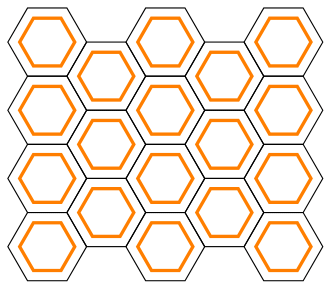
\includegraphics[width=6in]{fbi3.png}
$$
\ket{\psi} = \prod\limits_{\varhexagon} \left(\sum\limits_{i \in \varhexagon} b^{\dagger}_i \right) \ket{\mathbf{0}}
$$
\end{center}
\end{block}
      \vskip2ex
      \begin{block}{PEPS Construction of Honeycomb F.B.I.}

A wavefunction written as a product of local operators acting on a product state can be turned into a tensor network.


\begin{figure}[h]
\scalebox{1}{
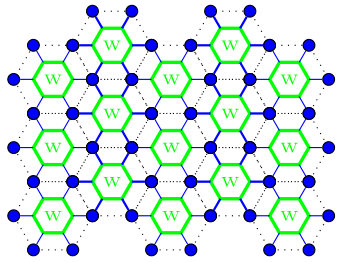
\includegraphics{FI_PEPS.png}
}
\end{figure}

Virtual W-state on each plaquette used to synchronize the creation operators in the sum $\sum\limits_{i \in \varhexagon} b^{\dagger}_i$
$$\vket{W} = \vket{000001}+\vket{000010}+\vket{000100}+\vket{001000}+\vket{010000}+\vket{100000}$$


\end{block}
       \vskip2ex
      \begin{block}{PEPS Construction of Honeycomb FBI}

\begin{columns}[T]
\begin{column}{0.5\textwidth}
\begin{figure}[h]
\scalebox{1.3}{
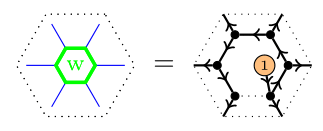
\includegraphics{diagrams/w_string.png}
}
\end{figure}
$$\vket{W} = \vket{100...}+...$$
\vskip-0.5cm
\bi 
\item W-State can be factored and put on hexagon sites
\item Each black directed string has either charge $0$ or $1$
\item Charge conserved
\ei 
\end{column}
\begin{column}{0.5\textwidth}
\begin{figure}[h]
\scalebox{1.5}{
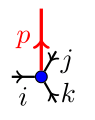
\includegraphics{diagrams/D_op.png}
}
\end{figure}
\vskip-0.3cm
\bi 
\item `Projects' the three virtual qubits coming into each vertex on to a state in physical Hilbert space
\item Physical state is either $\ket{0}, \ket{1}, \ket{2}, \ket{3}$
\item Charge conserved
\ei 
\end{column}
\end{columns}

\end{block}
      \vskip2ex
\end{column}

\begin{column}{\sepwid}\end{column}			% empty spacer column

\begin{column}{\midcolwid}	
      \begin{block}{Finite Size Analysis of Entanglement Spectra}
\begin{columns}[T]
\begin{column}{.5\textwidth}
        \begin{figure}[hbctp]
        \centering
        \includegraphics[width=\textwidth]{{EntanglementEnergyScaling.pdf}}
        %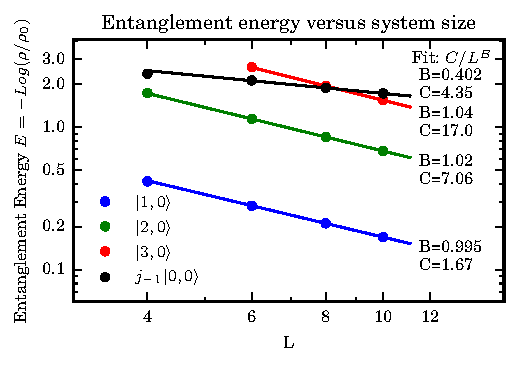
\includegraphics{{interpolatedboson/a10/plots/EntanglementEnergyScaling2.pdf}}
        %\caption{Power law fits for the lowest three states above the ground state at momentum zero and lowest two states at momentum 1 in Figure \ref{fig:sc-EEFinitesize}. The $1/L$ scaling is a signature of a gapless (entanglement) Hamiltonian. The labeling of the states $\ket{e, m}$ or $j_{-1} \ket{e, m}$ is explained in the CFT section below.}
        %\label{fig:sc-EEScaling}
        \end{figure}
        \bi 
        \item<1-> Low energy modes show gapless $1/L$ behavior
        \ei
\end{column}
\begin{column}{.5\textwidth}
\bi
\item Fix this to show topological entanglement entropy is 0
\ei
\end{column}
\end{columns}


\end{block}
      \vskip2ex
      \newcommand{\uL}{\mathbf{L_0}}
\newcommand{\bL}{\mathbf{\bar{L}_0}}
\begin{columns}[T]
\begin{column}{.6\textwidth}

\begin{block}{Conformal Charge}
	\begin{figure}[hbctp]
	\centering
	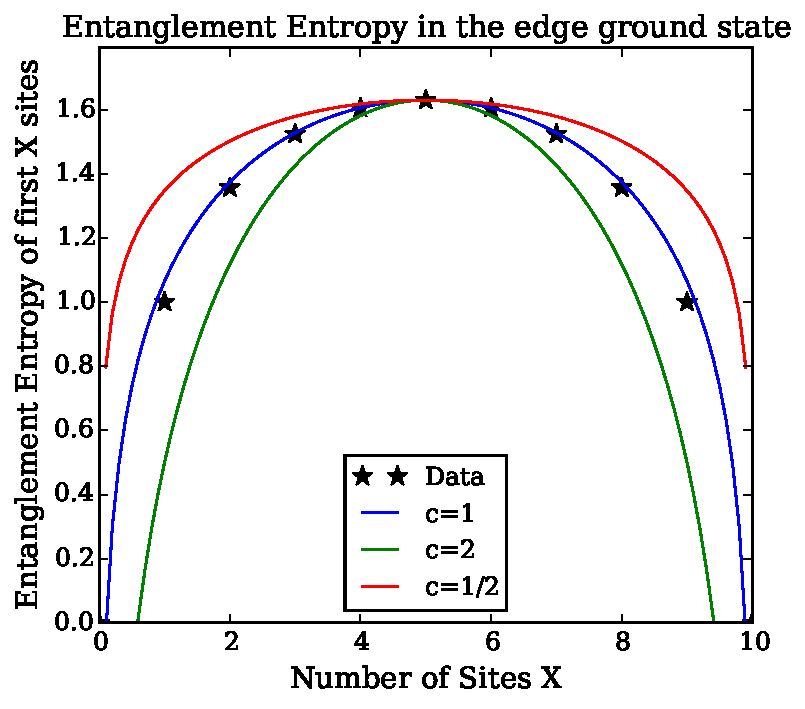
\includegraphics[width=\textwidth]{{interpolatedboson/a0/plots/edge_gs_EE.pdf}}
	%\caption{Entanglement entropy within the entanglement ground state of the soft-core boson state on $10$ sites. For comparison, the Cardy-Calabrese formula $S(x) = c/3 \log \sin( \pi x/L) + const.$ is shown with $c=\frac{1}{2}, 1,$ and $2$, with the $const.$ fixed by matching the maximum of the entanglement entropy data. $c=1$ is a good fit.}
	%\label{fig:hc-edge-gs-ee}
	\end{figure}
	\begin{empheq}[box={\mybluebox[4pt][4pt]}]{equation*}
	c = 1
	\end{empheq}
\end{block}
\end{column}
\begin{column}{.4\textwidth}
\begin{block}{Conformal Weights}
\vskip0.5cm
We can match the rescaled entanglement energies to the conformal weights of a free bosonic CFT.

%\begin{tabular*}{\columnwidth}{@{\extracolsep{\stretch{1}}}*{2}{c}@{}}
%\begin{tabularx}{\columnwidth}{|X|X|}
%\toprule
\small
\begin{align*}
	\mathbf{P} &=\frac{2\pi}{L}(\uL-\bL)  \\
	& = \frac{2\pi}{L}(em + n - \bar{n}) \\
	\widetilde{\mathbf{P}}&= em + n - \bar{n}\\ 
	\mathbf{H} &= \frac{2\pi}{L}(\uL+\bL)  \\
	&= \frac{2\pi}{L}(\frac{\kappa e^2}{2} + \frac{m^2}{2 \kappa} + \frac{n + \bar{n}}{2}) \\
	\widetilde{\mathbf{H}} &= \frac{L}{2 \pi \kappa}\mathbf{H} \\
&	= e^2 + \frac{m^2}{4 \kappa^2} + \frac{1}{\kappa}(n + \bar{n})
%\bottomrule
%\end{tabular*}
%\end{tabularx}
\end{align*}
\normalsize
\end{block}

%\begin{tabular}{lr}
%
%	$\mathbf{P} =\frac{2\pi}{L}(\uL-\bL)$ & 
%	$\frac{2\pi}{L}(em + n - \bar{n})$ \\
%	&
%	\\
%	$\widetilde{\mathbf{P}}$  &
%	$(em + n - \bar{n})$\\
%	& 
%	\\
%	$\mathbf{H} = \frac{2\pi}{L}(\uL+\bL)$ &
%	 $\frac{2\pi}{L}(\frac{\kappa e^2}{2} + \frac{m^2}{2 \kappa} + \frac{n + \bar{n}}{2})$ \\
%	&
%	 \\
%	$\widetilde{\mathbf{H}} = \frac{L}{2 \pi \kappa}\mathbf{H}$ &
%	 $e^2 + \frac{m^2}{4 \kappa^2} + \frac{1}{\kappa}(n + \bar{n})$       
%	\end{tabular}
	%\label{Table:EV}
	%\caption{Eigenvalues of states $\ket{e, m}_{n, \bar{n}}$.} 
	%\end{table}

\end{column}
\end{columns}

       \vskip2ex
      \begin{block}{CFT Identification of Gapless Entanglement Edge}
\begin{figure}[hbctp]
\begin{center}
\includegraphics[width=0.8\textwidth]{{EEIdentify.pdf}}
%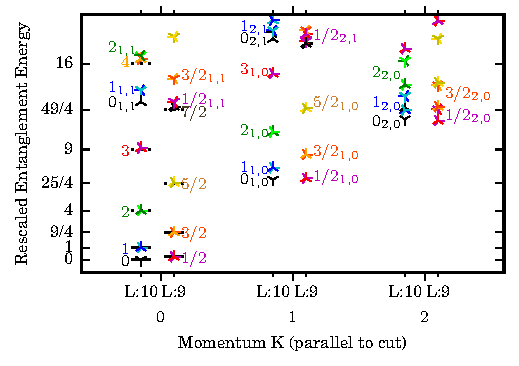
\includegraphics{{interpolatedboson/a10/plots/EEIdentify.pdf}}
\end{center}
%\caption{The identification of the states $\ket{e, m}_{n, \bar{n}}$ in the spectrum of the soft-core boson entanglement Hamiltonian. The label $e$ gives the U(1) charge. The labels $n$, $\bar{n}$ label the levels in the right or left-moving sectors of the Kac-Moody algebra. When the level $n$ is larger than 1, the level shows $Z(n)$ approximately degenerate states. The best estimate for the Luttinger parameter $\kappa = 1/6.4$ is given by the inverse of the energy of the $\ket{1, 0}_{1, 0}$ state. The label $m$ is 0 for all states shown - however, the primary states $\ket{e, m=\pm 1}$ can be seen centered around momentum $\pi$, with energies on the order of $1/(4\kappa^2)$.}
%\label{fig:primaries}
\end{figure}

\end{block}
      \vskip2ex%            
\end{column}

\begin{column}{\sepwid}\end{column}			% empty spacer column

\begin{column}{\rightcolwid}	
      \begin{block}{Detecting 1D SPT Order}
\vskip1cm
If $U_g$ is a global symmetry and $\ket{\psi}$ is translationally invariant, then the MPS representation satisfies:

\begin{figure}[h]
    \centering
    \scalebox{1}{
    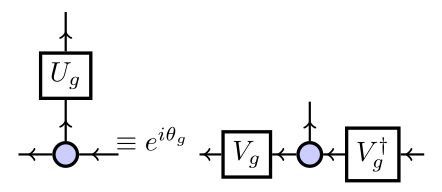
\includegraphics{group_sym.png}
    }
\end{figure}

Boundary conditions on a MPS can be represented by a matrix $B$ which acts like: 

\begin{figure}[h]
    \centering
    \scalebox{1}{
    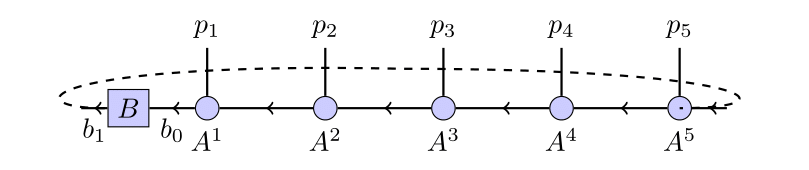
\includegraphics{mpsbc.png}
    }
\end{figure}

With PBC ($B=I$) , the group action leaves the state invariant. 

With OBC ($B = \ket{i}\bra{i}$), the group action rotates between states that differ only near the boundary; these edge states transform as $V_g \otimes V_g^{\dagger}$. 

$V_g$ represents the group projectively. Equivalence classes of projective representations (enumerated by $H^2(G; U(1))$) classify 1D SPT phases.

\end{block}
      \vskip2ex
      \begin{block}{Symmetry Protection of the Honeycomb FBI}

\vskip1cm

For the state on a cylinder with odd circumference, and the zig-zag entanglement cut defined in the upper left picture, we have the following:

\vskip1ex

\begin{tabular*}{\columnwidth}{@{\extracolsep{\stretch{1}}}*{5}{r}@{}}
\toprule
$\mathbf{G}$ & $\mathbf{U_g}$ & $\mathbf{\theta_g}$ & $\mathbf{V_g}$ &$\mathbf{V_g V^*_g}$ \\
\midrule
 $U(1)$ & & & & \\
 $\mathcal{\pi}$ & & & & \\
 $\mathcal{I}$ & & & & \\
 $\mathcal{\pi} \mathcal{I}$ & & & & \\
\bottomrule
\end{tabular*}

\vskip1ex
Since 
$$  
V_{\mathcal{\pi} \mathcal{I}} V_{\mathcal{\pi} \mathcal{I}}^* = -I \text{\quad or \quad } V_{\mathcal{\pi}} V_{\mathcal{I}} = - V_{\mathcal{I}} V_{\mathcal{\pi}},
$$ 

the representation is in the nontrivial class of 
\begin{empheq}[box={\mybluebox[2pt][2pt]}]{equation*}
H^2(\mathbb{Z}_2 \times \mathbb{Z}_2^{\mathcal{I}}; U(1)) = \mathbb{Z}_2.
\end{empheq}


\end{block}
       \vskip2ex
      \begin{block}{Relation to known 1D physics}
\bi 
\item Haldane insulator
\ei 
\end{block}
      \vskip2ex%
      \begin{block}{References}
\small{\begin{thebibliography}{99}

\bibitem{Kimchi} I. Kimchi, S. A. Parameswaran, A. M. Turner, F. Wang,
and A. Vishwanath, Featureless and non-fractionalized
mott insulators on the honeycomb lattice at 1/2 site filling,(2012), arXiv:1207.0498 [cond-mat.str-el].

\bibitem{Parameswaran} S. A. Parameswaran, A. M. Turner, D. P. Arovas, and
A. Vishwanath, Topological order and absence of band insulators at integer fillng in Non-Symmorphic crystals,
(2012), arXiv:1212.0557 [cond-mat.str-el]

\end{thebibliography}}
\vspace{0.75in}
\end{block}
      \vskip2ex%             
\end{column}

\begin{column}{\sepwid}\end{column}			% empty spacer column

\end{columns}
\end{frame}
\end{document}
%      \begin{block}{Altering Column Spans}
%        You can make columns that span multiple other columns relatively easily. Lengths are defined in the template that make columns look normal-ish if you want to use a four-column layout like this poster. If you want to use a different number of columns, you will have to modify those lengths accordingly at the top of the poster.tex file.
%        
%        In particular, near the top of the TeX file you will see lines that look like:
%        \begin{semiverbatim}
%          \hskip1ex\\setlength\{\\sepwid\}\{0.024\\paperwidth\}
%          
%          \hskip1ex\\setlength\{\\onecolwid\}\{0.22\\paperwidth\}
%          
%          \hskip1ex\\setlength\{\\twocolwid\}\{0.464\\paperwidth\}
%          
%          \hskip1ex\\setlength\{\\threecolwid\}\{0.708\\paperwidth\}
%        \end{semiverbatim}
%        
%        Set ``sepwid'' to be some small length somewhere near 0.025 (this is the space between columns). Then if $n$ is the number of columns you want, you should set
%        \begin{align*}
%          \text{onecolwid} & = \frac{1}{n}(1-(n+1)\times\text{sepwid}), \\
%          \text{twocolwid} & = 2\times\text{onecolwid} + \text{sepwid}, \\
%          \text{threecolwid} & = 3\times\text{onecolwid} + 2\times\text{sepwid}.
%        \end{align*}
%      \end{block}
%      \begin{columns}[t,totalwidth=\threecolwid]	% split up that three-column-wide column
%        \begin{column}{\onecolwid}
%%          \setbeamercolor{block title}{fg=red,bg=white}%frame color
%%          \setbeamercolor{block body}{fg=black,bg=white}%body color
%%          \begin{block}{Block Colours}
%%            For the standard blocks there are two colours; one for the title and one for the block body:\\
%%            \begin{semiverbatim}
%%              {\color{red}\\setbeamercolor}\{block title\}\newline \{fg=red,bg=white\}
%%            \end{semiverbatim}
%%            \begin{semiverbatim}
%%              {\color{red}\\setbeamercolor}\{block  body\}\newline \{fg=black,bg=white\}
%%            \end{semiverbatim}
%%            The \emph{fg} colour sets the text colour and \emph{bg} sets the background colour.
%%            For the normal blocks it makes no sense to use a background colour other than white. You \emph{can} change it, but it will look weird!
%%          \end{block}
%        \end{column}
%        \begin{column}{\onecolwid}
%          \setbeamercolor{block alerted title}{fg=black,bg=norange}	% frame color
%          \setbeamercolor{block alerted body}{fg=black,bg=white}		% body color
%          \begin{alertblock}{Alert Block Colours}
%            You can similarly modify the colours for alert blocks (but try not to overdo it):\\
%            \begin{semiverbatim}
%              {\color{red}\\setbeamercolor}\{block title\}\newline \{fg=black,bg=norange\}
%            \end{semiverbatim}
%            \begin{semiverbatim}
%              {\color{red}\\setbeamercolor}\{block  body\}\newline \{fg=black,bg=white\}
%            \end{semiverbatim}
%          \end{alertblock}        
%        \end{column}
%        \begin{column}{\onecolwid}
%          \begin{block}{References}
%            Some references and a graphic to show you how it's done:
%            
%		        \small{\begin{thebibliography}{99}
%		        \bibitem{KLPL06} D.~W. Kribs, R. Laflamme, D. Poulin, M. Lesosky, Quantum Inf. \& Comp. \textbf{6} (2006), 383-399.
%		        \bibitem{zanardi97} P. Zanardi, M. Rasetti, Phys. Rev. Lett. \textbf{79},  3306 (1997).
%		        \end{thebibliography}}
%			      \vspace{0.75in}
%			      \begin{center}
%			        
\includegraphics[width=5in]{Microsoft-Research.jpg}
%			      \end{center}
%		      \end{block}
%        \end{column}
%      \end{columns}
%      \vskip2.5ex